\documentclass[11pt, a4paper]{article}

\usepackage{german}
\usepackage{graphicx} 
\usepackage[utf8]{inputenc}
\usepackage{fancyhdr}
\usepackage{changepage}
\usepackage[onehalfspacing]{setspace}
\usepackage{ragged2e}
\usepackage{ amssymb, amsmath, amsthm, dsfont }
\usepackage[width = 18cm, top = 2.5cm, bottom = 3cm]{geometry}
\usepackage{extarrows}
% --------- Variabel, auf jedem Blatt ändern!
\newcommand{\blattnummer}{6}
\newcommand{\datum}{18. Juni 2017}
	% Punktezahlen & Summe
\newcommand{\p}{10}
\newcommand{\pp}{5}
\newcommand{\ppp}{5}
\newcommand{\pppp}{}
\newcommand{\sump}{20}
% --------- Macros

\newcommand{\myTitleString} {}
\newcommand{\myAuthorString} {}
\newcommand{\mySubTitleString} {}
\newcommand{\myDateString} {}

\newcommand{\myTitle}[1] {\renewcommand {\myTitleString}{#1}}
\newcommand{\mySubTitle}[1] {\renewcommand {\mySubTitleString}{#1}}
\newcommand{\myAuthor}[1] {\renewcommand{\myAuthorString}		{#1}}
\newcommand{\myDate}[1] {\renewcommand{\myDateString}{#1}}

\newcommand{\makeMyTitle}
{
\pagestyle{fancy}
\fancyhead[L]
{
\begin{tabular}{l}
\myTitleString
\\ \mySubTitleString 
\\ \myDateString
\end{tabular}
} 			
\fancyhead[C]{}
\fancyhead[R]{\myAuthorString}
\fancyfoot[C]{\thepage}
}

\setlength{\headheight}{45pt}

\makeatletter
\renewcommand*\env@matrix[1][*\c@MaxMatrixCols c]{%
  \hskip -\arraycolsep
  \let\@ifnextchar\new@ifnextchar
  \array{#1}}
\makeatother

    % args: Aufgabennummer, erreichbare Punkte
\newcommand{\aufgabe}[2] {\section*{Aufgabe \blattnummer.#1 (Punkte:\qquad/#2)}}
\newcommand{\aufgabenteil}[1] {\textbf{(#1)}}
% ---------
%\setlength{\parindent}{0pt}
\begin{document}

\myTitle{\textsc{Datenbanken und Informationssysteme}}
\mySubTitle{Übung \blattnummer}
\myDate{\datum}
\myAuthor
{
\begin{tabular}{l l}
359109, &Michelle Milde\\
356148, &Philipp Hochmann\\
356092, &Daniel Schleiz
\end{tabular}
}
\makeMyTitle

\hfill
\begin{tabular}{|c|c|c|c|}\hline
   1 & 2 & 3 & $\sum$\\\hline
  	 \qquad/\p & \qquad/\pp & \qquad/\ppp & \qquad/\sump\\\hline % abhängig vom Übungsblatt
 \end{tabular}
\hfill Korrigiert am:\underline{\hspace{3cm}}
\hfill
\vspace*{30pt}


\aufgabe{1}{\p}
\begin{enumerate}
\item Bestimme die \textit{kanonische Überdeckung} zu $F$:
\begin{enumerate}
\item \textit{Linksreduktion}:\\
$A \rightarrow D$ nicht linksreduzierbar, da $D \notin \emptyset^+$. $ABC \rightarrow E$ ist linksreduzierbar: Zunächst ist $\{ B,C\}^+=\{B,C\}$, also darf man $A$ nicht weglassen.
Da aber $E \in\{ A,C\}^+=\{ A,C,D,G,B,E\}$ und $E \in \{ A\}^+= \{ A,D,E,B\}$ (mit $A \rightarrow D$ und $D \rightarrow BE$), lässt sich $ABC \rightarrow E$ reduzieren auf $A
\rightarrow E$. $AC \rightarrow G$ lässt sich nicht reduzieren, da $G \notin \{ A\}^+$ und $G \notin \{ C\}^+=\{ C\}$. Die restlichen FDs ebenfalls nicht, da nur ein Attribut auf der linken
Seite und die Attributhülle der leeren Menge leer ist.\\
Es ergibt sich als Zwischenergebnis die Menge $F' = \{ A \rightarrow D, A \rightarrow E, AC \rightarrow G, D \rightarrow BE, E \rightarrow B, G \rightarrow CE\}$ von FDs.
\item \textit{Rechtsreduktion}:\\
$A \rightarrow D$ ist nicht rechtsreduzierbar, da $D$ nur in dieser FD auf der rechten Seite auftritt und somit nicht in der Attributhülle von $A$ liegt mit der reduzierten FD. $A \rightarrow E$
ist rechtsreduzierbar, da $\{ A\}^+= \{ A,D,B,E\}$ mittels $A \rightarrow D \rightarrow BE$, ersetze also durch $A \rightarrow \emptyset$. $AC \rightarrow G$ nicht reduzierbar, da $G$
nur in dieser FD auf der rechten Seite. $D \rightarrow BE$ ist reduzierbar: Ersetze durch $D \rightarrow E$, da mit $D\rightarrow E$ und $E \rightarrow B$ das Attribut $B$ in der Hülle von
$D$ liegt. Nicht weiter reduzierbar, da die Attributhülle von $D$ sonst nur aus $D$ bestünde, insbesondere $E$ nicht drin. $E \rightarrow B$ nicht reduzierbar, da sonst $B$ nicht in der
Attributhülle von $E$ ist, weil diese leer wäre. $G \rightarrow CE$ ist auch nicht reduzierbar, da sonst das entfernte Attribut auf der rechten Seite jeweils nicht mit in der Hülle von $G$ läge.\\
Neues Zwischenergebnis: $F''=\{ A \rightarrow D, A \rightarrow \emptyset, AC \rightarrow G, D \rightarrow E, E \rightarrow B, G \rightarrow CE\}$.
\item Entferne FDs der Form $\alpha \rightarrow \emptyset$, Anwendung der Vereinigungsregel für FDs:\\
Es ergibt sich die kanonische Überdeckung $F_c=\{ A \rightarrow D, AC \rightarrow G, D \rightarrow E, E \rightarrow B, G \rightarrow CE\}$.
\end{enumerate}

\item Erstelle Relationenschemata (für jede FD in $F_c$):
\begin{itemize}
\item $R_1=(\{ A,D\},\{ A \rightarrow D\})$
\item $R_2=(\{ A,C,G\},\{ AC \rightarrow G\})$
\item $R_3=(\{ D,E\},\{ D \rightarrow E\})$
\item $R_4=(\{ E,B\},\{ E \rightarrow B\})$
\item $R_5=(\{ G,C,E\},\{ G \rightarrow CE\})$
\end{itemize}
Nun enthält bereits das Relationenschema $R_2$ den Schlüsselkandidaten $\{ A,C\}$, weshalb keine Schemata mehr hinzuzufügen sind. (Der andere Schlüsselkandidat wäre $\{ A,G\}$).
Da keine Attributmenge eines Schemas Teilmenge eines anderen Schemas ist, muss keines eliminiert werden. Somit liegt die gewünschte 3NF-Zerlegung vor.

\end{enumerate}



\aufgabe{2}{\pp}
\aufgabenteil{a}
\begin{adjustwidth}{20pt}{20pt}
\begin{tt}
SELECT DISTINCT arzt.name\\
FROM arzt, patient, behandlung, medikament\\
WHERE patient.name = 'Peter Parker'\\
\null\qquad AND patient.patient\_id = behandlung.patient\\
\null\qquad AND arzt.arzt\_id = behandlung.arzt\\
\null\qquad AND behandlung.medikament = medikament.medikament\_id\\
\null\qquad AND medikament.name = 'Palladium'\\
\end{tt}
\end{adjustwidth}
\aufgabenteil{b}
\begin{adjustwidth}{20pt}{20pt}
\begin{center}
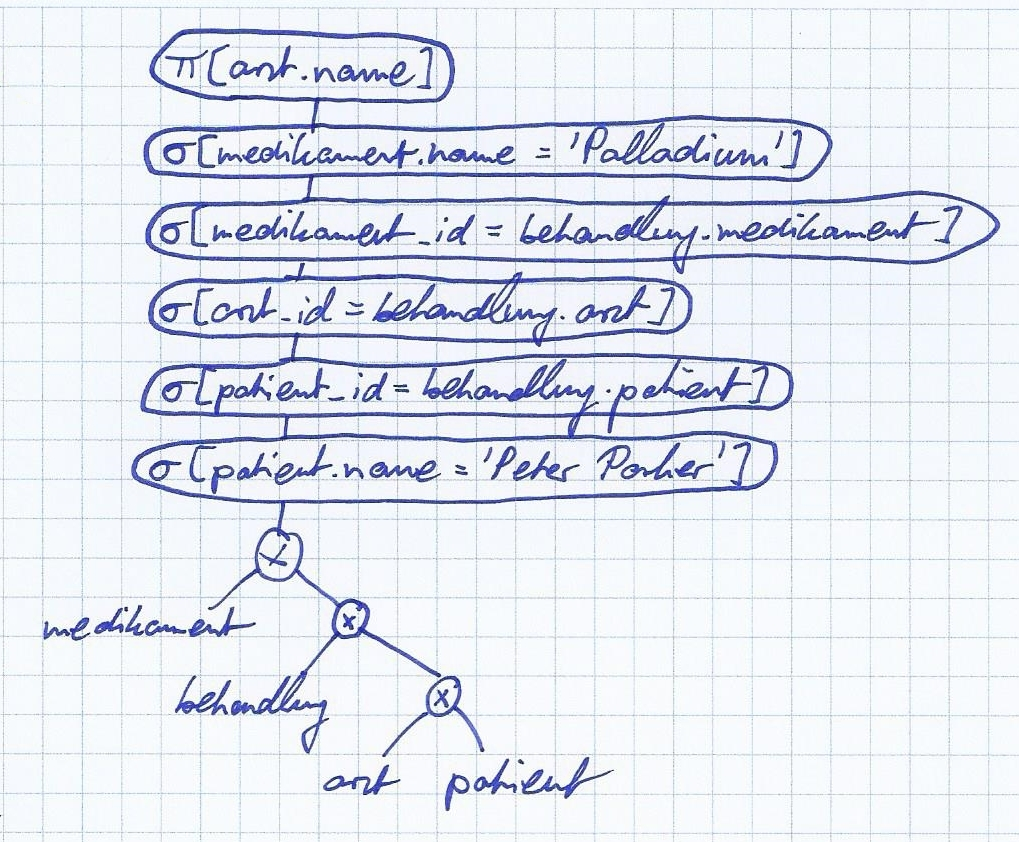
\includegraphics[width=0.5\textwidth]{a2b.jpg}
\end{center}
\end{adjustwidth}
\aufgabenteil{c}
\begin{adjustwidth}{20pt}{20pt}
\begin{center}
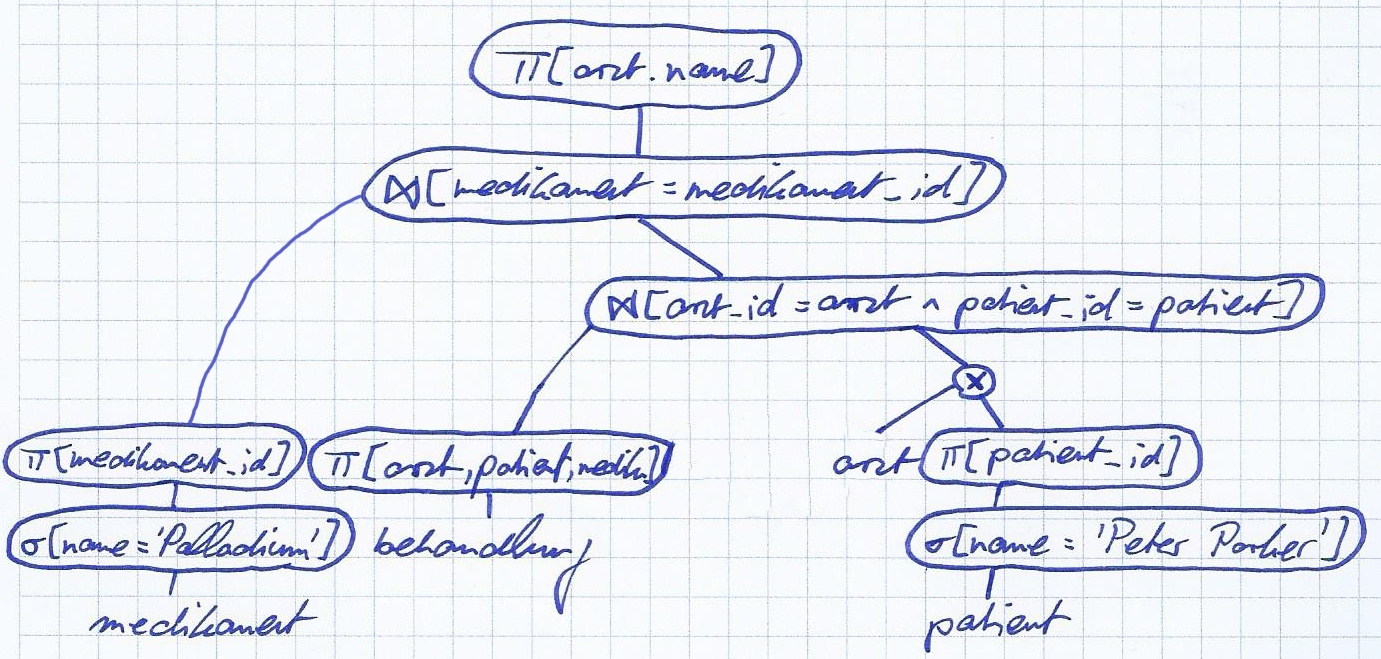
\includegraphics[width=0.5\textwidth]{a2c.jpg}
\end{center}
\end{adjustwidth}



\aufgabe{3}{\ppp}
\begin{adjustwidth}{20pt}{20pt}

\end{adjustwidth}


% --------
\end{document}
